\documentclass[12pt,a4paper]{article}

% Packages
\usepackage[utf8]{inputenc}
\usepackage[T1]{fontenc}
\usepackage[english]{babel}
\usepackage{amsmath, amssymb}
\usepackage{graphicx}
\usepackage{enumitem}
\usepackage{geometry}
\geometry{margin=2.5cm}
\usepackage{float}
\usepackage{caption}

\title{Problem R28 (Revised): Viscous Flow in Combined Pipe and Hull System}
\author{}
\date{}

\begin{document}

\maketitle

\section*{Scenario}

A research vessel uses a hybrid propulsion system composed of:
\begin{itemize}
    \item a conventional propeller system, and
    \item a water discharge system that ejects seawater through two \textbf{serial} pipe sections (see sketch).
\end{itemize}

The system is designed such that all pipe flow is \textbf{tripped to turbulent regime at the inlet}. The outer hull flow is also assumed \textbf{fully turbulent}, avoiding laminar-transition complexity.

\medskip
Assume seawater at density $\rho = 1025\,\mathrm{kg/m^3}$ and kinematic viscosity $\nu = 1.1 \times 10^{-6}\,\mathrm{m^2/s}$.

\paragraph{Pipe Sections:}
\begin{itemize}
    \item Section A: length $L_A = 30\,\mathrm{m}$, diameter $D_A = 0.3\,\mathrm{m}$, roughness $k_A = 0.3\,\mathrm{mm}$
    \item Section B: length $L_B = 20\,\mathrm{m}$, diameter $D_B = 0.2\,\mathrm{m}$, roughness $k_B = 1.2\,\mathrm{mm}$
\end{itemize}
Total volumetric flow rate: $Q = 0.08\,\mathrm{m^3/s}$

\paragraph{Hull Geometry:}
\begin{itemize}
    \item Length $L = 85\,\mathrm{m}$
    \item Draft $T = 6\,\mathrm{m}$
    \item Roughness $k_s = 4\,\mathrm{mm}$
\end{itemize}
Assume the \textbf{wetted area} is approximately $A = 2 \cdot L \cdot T$ (i.e. both vertical sides only).

Ship velocity: $V = 9\,\mathrm{m/s}$ \\
Propeller efficiency: $\eta_S = 0.78$

\section*{Tasks}
\begin{enumerate}[label=\alph*)]
    \item Calculate the \textbf{mean velocity} in each pipe section based on $Q$ and cross-sectional area.

    \item Compute the \textbf{Reynolds number} for each pipe and confirm turbulent regime.

    \item Using the Darcy-Weisbach equation, determine the \textbf{total pressure loss} $\Delta p_V$ over the pipe system:
    \[
    \Delta p_V = \sum_i \left( \lambda_i \cdot \frac{L_i}{D_i} \cdot \frac{\rho}{2} \cdot \bar{u}_i^2 \right)
    \]
    where the friction factor $\lambda$ for \textbf{fully rough turbulent flow} is given by:
    \[
    \frac{1}{\sqrt{\lambda}} = 1.74 - 2 \log_{10}\left( \frac{2k}{D} \right)
    \]
    \textit{Hint: Alternatively, you may use the pipe friction diagram provided (Lecture Notes p.119).}

    \item Compute the \textbf{friction coefficient} for the hull using:
    \[
    c_f = \left(1.89 + 1.62 \cdot \log_{10}\left(\frac{L}{k_s}\right)\right)^{-2.5}
    \]
    and determine the \textbf{total frictional resistance} over the wetted area.
    
    \textit{Assume outer flow is fully turbulent. You may also refer to the flat plate diagram (Lecture Notes p.164).}

    \item Calculate the \textbf{total effective power} required to:
    \begin{itemize}
        \item overcome the pipe pressure losses, and
        \item overcome hull friction resistance.
    \end{itemize}
    Then determine the \textbf{required engine power} accounting for the propeller efficiency:
    \[
    P = \frac{F \cdot V + Q \cdot \Delta p_V}{\eta_S}
    \]
    \textit{If unable to solve previous tasks, assume: $\lambda_A = 0.025$, $\lambda_B = 0.035$, $c_f = 0.0035$}
\end{enumerate}

\begin{figure}[H]
    \centering
    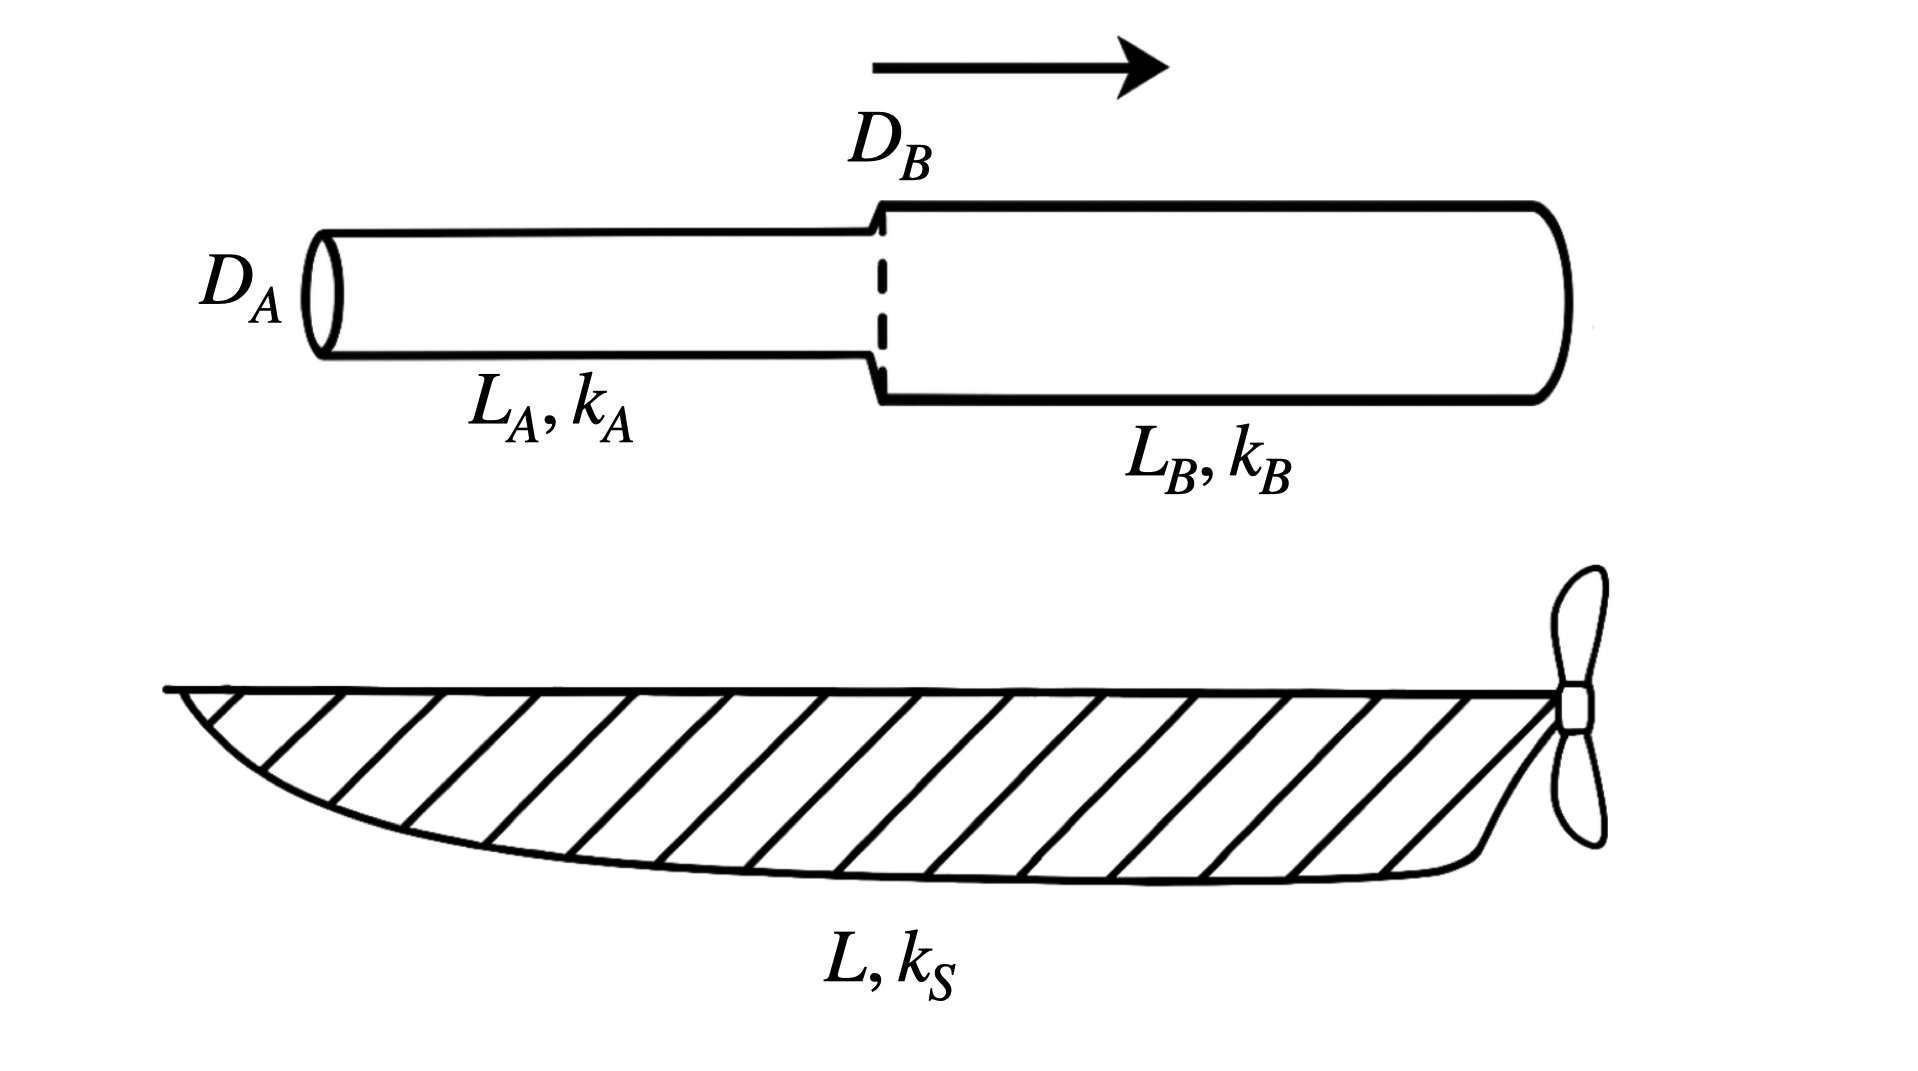
\includegraphics[width=0.85\textwidth]{HullSketch.png} % Replace with actual sketch file
    \caption{Sketch of the vessel and serial pipe discharge system (not to scale)}
\end{figure}

\end{document}
